\section{Design}
\label{sec:design}
\subsection{Probabilistic Minimum}
Starting with the Space Saving algorithm as a baseline, we first settled on probabilistic sampling as a way to make finding the minimum element more efficient, rather than linearly searching the entire table. As long as a flow with a low enough frequency is evicted when a new flow is encountered, larger flows will still be preserved in the table. As Figure~\ref{fig:probMin} shows, sampling as few as 4 elements probabilistically ensures that only elements in the lowest quintile will be evicted. Drawing from HashPipe, we implemented this optimization using a hash table pipeline, as the number of stages equals the number of elements probabilistically sampled. If there are four stages in the pipeline, the minimum of the four flows encountered (one per stage) will be a candidate for eviction. 
\begin{figure}[t]
  \centering
    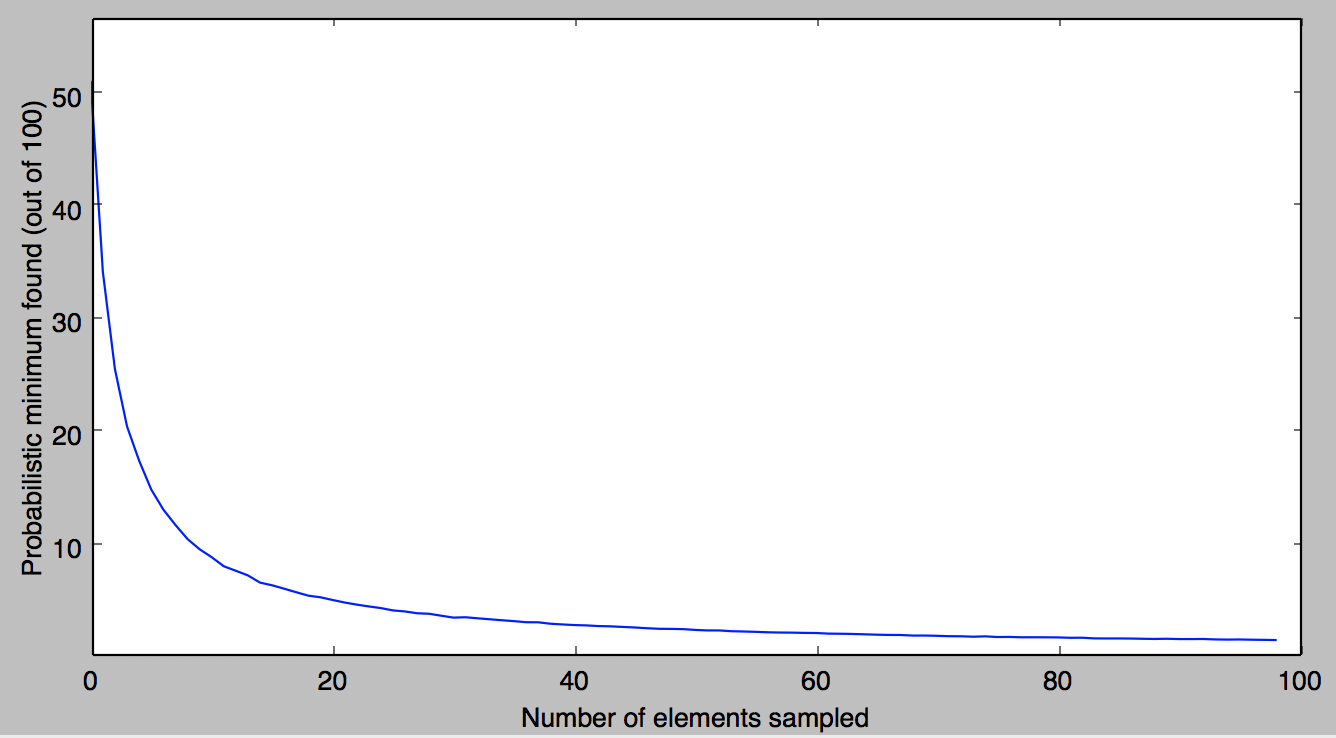
\includegraphics[scale=0.32]{probMin}
     \caption{The minimum of a randomly selected set of elements approaches the true minimum}
     \label{fig:probMin}
\end{figure}
\subsection{Randomized Assignment}
HashPipe, as the name suggests, features a consistent hashing scheme whereby each stage uses an independent hash function and subsequent repeated flows consistently hash to the same location within each stage. This scheme is intended to reduce the number of duplicate flows occupying space in the pipeline and consolidate their counts. However, we experimentally determined that using a random function to determine flow assignment within the first stage resulted in improvements in accuracy of nearly 50 percent.
\subsection{Logarithmic Admission Policy}
One of the major flaws with HashPipe is the fact that, as with Space Saving, every flow will always be admitted into the pipeline, even if it will never reoccur. In streams with many small flows, accuracy suffers as heavy hitters near the minimum threshold are evicted by small newly encountered flows. Therefore, we introduced a modified admission policy inspired by RAP, but instead of making the probability of admission inversely proportional to the frequency of the minimum counter, we used a log function to dampen extremely low admission probabilities. We introduced a log function to counteract one of the systematic errors with RAP: denying admission to new heavy hitters. This way, flows with high frequencies are still protected, but smaller flows have a larger probability of being evicted. We tested two potential solutions to this problem, both of which restrict admission to the table.

In Front Rejection (AKA The Bouncer), packets are randomly assigned a slot in the first stage. If empty, the packet is inserted and the frequency is set to 1. If the slot contains a packet with the identical source IP address, the frequency is incremented. Otherwise, the packet evicts the resident of the slot with probability $p = 1 / (5*log(c_m + 1))$, where $c_m$ is the frequency count of the flow in the slot. This is easy to implement, and it saves a lot of computational resources further down the pipeline, since on average 90 percent of packets will be refused admission to the pipeline. However, it is not necessarily accurate because the probability of admission is determined by only the flow randomly compared to in the first stage of the pipeline. This flow is not guaranteed to the be the minimum, but it is likely to be an average flow, which turns out to be an adequate compromise.

In Back Rejection (AKA The Interview), all packets are admitted to the entrance of the pipeline and proceed through all stages of the pipeline. However, rather than always evicting the minimum of the flows encountered throughout the pipeline to make way for the new flow, a calculation is made at the end of the pipeline. With probability $p = 1 / (5*log(c_m + 1))$, the minimum flow is evicted, otherwise the minimum flow is inserted back into the first stage, retroactively denying admission to the newly encountered flow located in the first stage. 
\begin{figure}[t]
  \centering
    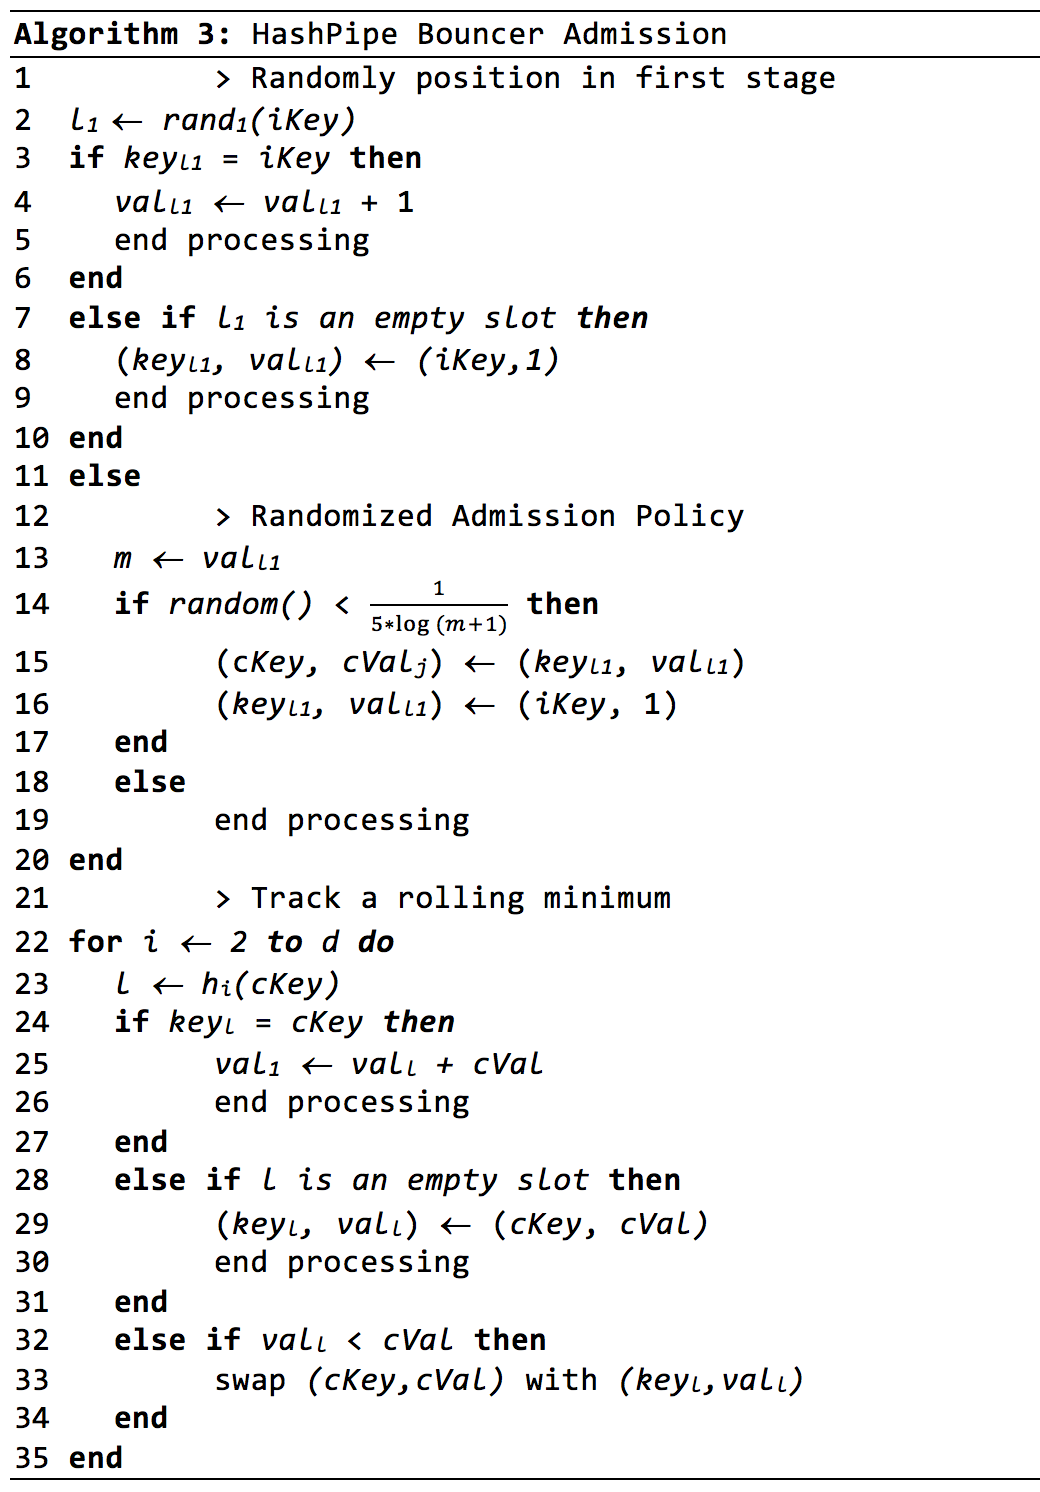
\includegraphics[scale=0.42]{alg3}
     \label{fig:bp-image}
\end{figure}